\documentclass[12pt, a4paper, twoside]{article}

\usepackage{a4wide}
\usepackage[USenglish, ngerman]{babel}
\usepackage[latin1]{inputenc}
\usepackage[T1]{fontenc}
\usepackage{makeidx}
\usepackage{url}
\usepackage{doc}
\usepackage{graphicx}
\usepackage{lmodern} 
\usepackage{amsmath}
\usepackage{amssymb}
\usepackage{hyperref}
\usepackage{fancyheadings}
\usepackage{amsfonts}
\usepackage{amsthm}
\usepackage{color}
\usepackage{stmaryrd}
\newcommand{\rf}{\color{red}}
\newcommand{\wf}{\color{white}}
\newcommand{\tf}{\color{black}}


%Kopf- und Fußzeile
\usepackage{fancyhdr}
\pagestyle{fancy}
\fancyhf{}

%Kopfzeile links bzw. innen
\fancyhead[L]{\scshape\leftmark}
%Linie oben
\renewcommand{\headrulewidth}{0.5pt}

%Fußzeile links bzw. innen
\fancyfoot[C]{\thepage}
%Linie unten
\renewcommand{\footrulewidth}{0.5pt}
\emergencystretch=3em

% Umgebungen für Sätze usw.
\newtheorem{satz}{Satz}
\newtheorem{defi}[satz]{Definition}
\newtheorem{bez}[satz]{Bezeichnung}
\newtheorem{bsp}[satz]{Beispiel}
\newtheorem{thm}[satz]{Theorem}
\newtheorem{kor}[satz]{Korollar}
\newtheorem{prob}[satz]{Problem}
\newtheorem{lem}[satz]{Lemma}

\numberwithin{equation}{section}
\begin{document}


\begin{titlepage}
\pagenumbering{roman}
\begin{center}
\vspace{1em}
\textbf{
\Large Heinrich-Heine-Universit"at D"usseldorf\\
\smallskip
\Large Institut f"ur Mathematik\\
\smallskip}

\vspace{3em}
{\Huge Seminarpaper\\}
\vspace{3em}
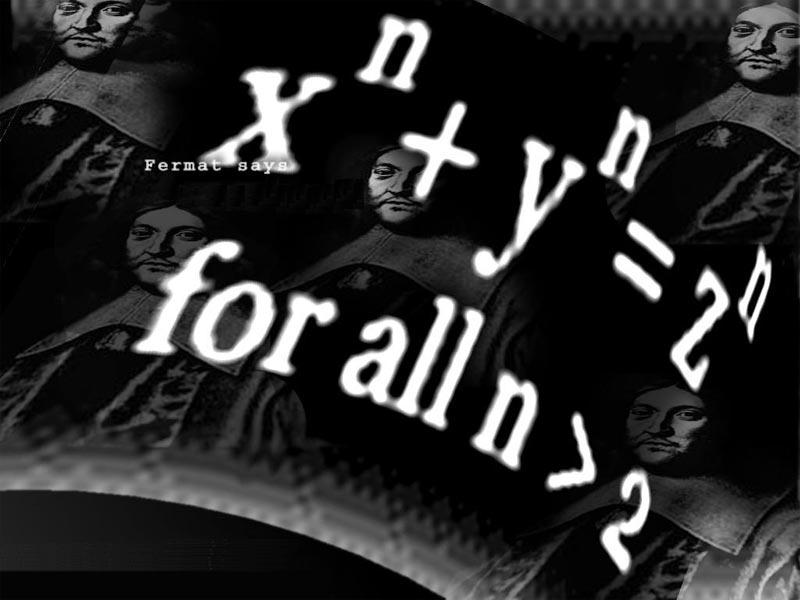
\includegraphics[height=6cm]{a.jpg}\\
\vspace{4em} {\Huge Fermat's Last Theorem}
\end{center}

\vfill

\begin{center}
{\large
\begin{tabular}[l]{ll}
Name: & Alina Elterman\\
Matrikelnummer: & 1810231\\
Abgabedatum: & 02.12.2010
\end{tabular}
}
\end{center}
\end{titlepage}
\newpage
\thispagestyle{empty}
\tableofcontents
\newpage
\thispagestyle{empty}
\phantomsection
\listoffigures
\newpage
\pagenumbering{arabic}
\setcounter{page}{1}
\section{Introduction}
Over more than threehundred years was Fermat's Last Theorem an unsolved mathematic conjecture. Although the statement can be understood by nearly every child, the proof couldn't been found by many genious scientists. The proof scetches developed together with the development of mathematics, and the history of the solution is closely related to the history of mathematics itself. Prior to its 1995 proof it was in the Guinness Book of World Records for ''most difficult math problem''.\\
This paper is structed into two parts. In the first I'll give the historical background and the progression in the proof, which were made untill the propositions of my talk.\\
The second part is about the four theorems, which I describe and proof. I will expecially point out the meaning of them to the developement of the proof.
\section{The Historical Content}
\subsection{Pythagorean Theorem}
Once upon a time in Greece lived a man named Pythagoras. One of his main interests was Mathematics, so he traveled across the world in 500's BC and tried to collect all the knowledge together. He find a very interesting fact, and afterwards the people named this after him. The statement of the Theorem was discovered on a Babylonian tablet circa 1900-1600 B.C. and it says:
$$x^2+y^2=z^2$$
It can be easy visualised by:\\
\newline
\begin{center}
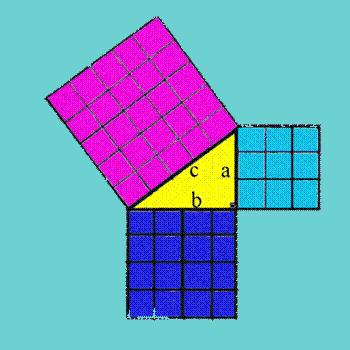
\includegraphics[height=4cm]{b.jpg}
\newline
\end{center}
The geometrical interpretation is that the number of squares for the ancles must the same as the numer of squares for the hypotenuse if the triangle is right. Pythagoras was only interested in integer solutions and also showed that there exist infinitely many of them. The details were shown by Janine Haas in the first talk.
\subsection{Fermat's Heritage}
\begin{center}
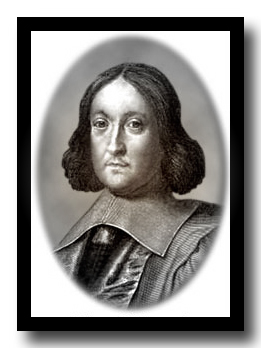
\includegraphics[height=13cm]{fermat.jpg}
\newline
\end{center}
Pierre de Fermat lived in the 17th century in France. At this time Mathematics were not highly esteemed, so he studied and practised Law, but his passion stayed by the Mathematics. He didn't like to share his ideas, and so he wrote them offen as comments in books, which were at first his only source. The most important of them were written in the 1621 edition of the Arithmetica of Diophantus. When he died his son realised the importance of his fathers sripts and published them. After years the mathematicians all over the world solved all proofs Fermat suggested in his comments, except: ''I have discovered a truly marvelous proof that it is impossible to separate a cube into two cubes, or a fourth power into two fourth powers, or in general, any power higher than the second into two like powers. This margin is too narrow to contain it.'' In math discription it means:\\
$$There exist no solution for x^n+y^n=z^n, n>2.$$
So this one get the honour of beeing Fermat's Last Theorem. Rightly!
\newpage
\section{The Proof}
The case $n=4$ was proven by Fermat himself. Fermat uses the technique of infinite descent to show that the area of a right triangle with integer sides can never equal the square of an integer. His proof is equivalent to demonstrating that the equation $$x^4 - y^4 = z^2$$ has no primitive solutions in integers (no pairwise coprime solutions). In turn, this proves Fermat's Last Theorem for the case n=4, since the equation $$a^4 + b^4 = c^4$$ can be written as $$c^4-b^4 = (a^2)^2$$. 
\subsection{Proof of Fermat's Last Theorem for specific exponents}
\subsection{Kevin Ondo: The case $x^4+y^4=z^4$ and Sophie Germain's Theorem}
\begin{satz}[1.Satz von Sophie Germain]
Ist $p$ Prim und $a \in \mathbb{N}$ teilerfremd zu $p$, so gilt:\\
$$a^{p-1} \equiv 1 \pmod  p$$
\end{satz}
\begin{defi}
Eine Primzahl $p$ heisst Sophie-Germain-Primzahl (SGP), wenn sie ungerade ist und auch $q=2p+1$ eine Primzahl ist.
\end{defi}
\begin{bsp}
p=3 und q=7 $\rightarrow$ $3 \in SGP$\\
p=7 und q=15, $q \notin Prim$ $\rightarrow$ $7 \notin SGP$
\end{bsp}
\begin{thm}
Sei $p$  eine SGP. Dann gibt es keine L"osung der Gleichung $$x^p+y^p+z^p=0$$ f"ur $x,y,z \in\mathbb{Z}$ mit $p\nmid xyz$ und $x,y,z$ paarweise teilerfremd.
\end{thm}
\begin{proof}
Sei $q=2p+1$, $(x,y,z)$ eine nichttriviale L"osung.\\
Aus $x^p+y^p+z^p=0$ $\Rightarrow$ $x^p+y^p=-z^p
=xy^{p-1}-x^2y^{p-2}+ \cdots -x^{p-1}y+x^p+y^p-xy^{p-1}+x^2y^{p-2}+ \cdots +x^{p-1}y=x(y^{p-1}-xy^{p-2}+ \cdots x^{p-1})+y(y^{p-1}-xy^{p-2}+ \cdots x^{p-1})=(x+y)\underbrace{(y^{p-1}-xy^{p-2}+ \cdots x^{p-1})}_{\alpha}$ wegen $p\nmid z$ gilt $p \nmid (x+y)$.\\
Sei $r$ eine Primzahl des ggT von $(x+y)$ und $\alpha$. Dann gilt $r \neq p$ und $x \equiv -y \pmod r$, weil $p \nmid (x+y)$ und $r|(x+y)$.\\
\newpage
\begin{tabular}{lll}
Daher gilt:& $0$ & $\equiv y^{p-1} -xy^{p-2} + \cdots + x^{p-1} \pmod r$\\&&$\equiv y^{p-1}-(-y)y^{p-2}+ \cdots + (-y)^{p-1}$\\&&$\equiv y^{p-1}+y^{p-1}+ \cdots + y^{p-1} \pmod 1$\\
&$0$ & $\equiv py^{p-1} \pmod r$ $\Leftrightarrow r | py^{p-1} $ da $r \nmid p$ \\&& $\Rightarrow r|y$ da $r| (x+y)$ und $r|y$ folgt $r|x$\\ && $\Rightarrow r|z$  WIDERSPRUCH!!!!\\
\end{tabular}
\newline
\newline
$(-y)^p=x^p+y^p$ und $(-x)^p=y^p+z^p$ analog.\footnote{Frage: Warum $x+y=a^p$ f"ur ein $a,t \in \mathbb{Z}$?\\
L"osung: Primfaktorzerlegung}\\
\newline
$q=2p+1 \Rightarrow q-1=2p$ so $a^{q-1}= \begin{cases}

  1 \pmod q,  & q \nmid a,\\
  0 \pmod q, & q \nmid a, q|a.
\end{cases}$ ...\\
\newline
F"ur $q>3$ gilt: $x^p+y^p+z^p = 0 \equiv 0 \pmod q$
\begin{itemize}
\item $q | 2x = x+y+x+z-y-z= a^p+b^p-c^p \equiv \pmod q$\\
\item $q|x$ $a^p=x+y$ wenn $q|a^p \Rightarrow q|y $ WIDERSPRUCH!\\ $\Rightarrow q|c^p$ 
\item $q|(a^p+b^p)=(x+y+x+z)=(2x+y+z) \Rightarrow y+z \equiv 0 \pmod q$
\end{itemize}
$s^p = z^{p-1}-yz^{p-2}+ \cdots + y^{p-1} | y \equiv -z \pmod q = py^{p-1} \pmod q$\\
$s^p \equiv \pm1 \pmod q , q\nmid y$.\\
\newline 
$py^{p-1} \equiv \pm1 \pmod q$\\
\newline
$(-z)^p = (x+y)t^p$ und $\pm1 \equiv y^p \equiv yt^p \pmod q$ mit $q \nmid y$\\
$q=2p+1 \Rightarrow p \not\equiv \pm 1 \pmod q$
\end{proof}

After Fermat proved the special case n = 4, the general proof for all n required only that the theorem be established for all odd prime exponents.[46] In other words, it was necessary to prove only that the equation ap + bp = cp has no integer solutions (a, b, c) when p is an odd prime number. This follows because a solution (a, b, c) for a given n is equivalent to a solution for all the factors of n. For illustration, let n be factored into d and e, n = de. The general equation

    an + bn = cn

implies that (ad, bd, cd) is a solution for the exponent e

    (ad)e + (bd)e = (cd)e

Thus, to prove that Fermat's equation has no solutions for n > 2, it suffices to prove that it has no solutions for at least one prime factor of every n. All integers n > 2 contain a factor of 4, or an odd prime number, or both. Therefore, Fermat's Last Theorem can be proven for all n if it can be proven for n = 4 and for all odd primes p.
In the two centuries following its conjecture (1637-1839), Fermat's Last Theorem was proven for three odd prime exponents p = 3, 5 and 7. The case p = 3 was first stated by Abu Mahmud Khujandi (10th century), but his attempted proof of the theorem was incorrect.[47] In 1770, Leonhard Euler gave a proof of p = 3,[48] but his proof by infinite descent[49] contained a major gap.[50] However, since Euler himself had proven the lemma necessary to complete the proof in other work, he is generally credited with the first proof.[51] Independent proofs were published[52] by Kausler (1802)[25], Legendre (1823, 1830),[27][53] Calzolari (1855),[54] Gabriel Lamé (1865),[55] Peter Guthrie Tait (1872),[56] Günther (1878),[57] Gambioli (1901),[36] Krey (1909),[58] Rychlík (1910),[41] Stockhaus (1910),[59] Carmichael (1915),[60] Johannes van der Corput (1915),[61], Axel Thue (1917),[62] and Duarte (1944).[63] The case p = 5 was proven[64] independently by Legendre and Peter Dirichlet around 1825.[65] Alternative proofs were developed[66] by Carl Friedrich Gauss (1875, posthumous),[67] Lebesgue (1843),[68] Lamé (1847),[69] Gambioli (1901),[36][70] Werebrusow (1905),[71] Rychlík (1910),[72] van der Corput (1915),[61] and Guy Terjanian (1987).[73] The case n = 7 was proven[74] by Lamé in 1839.[75] His rather complicated proof was simplified in 1840 by Lebesgue,[76] and still simpler proofs[77] were published by Angelo Genocchi in 1864, 1874 and 1876.[78] Alternative proofs were developed by Théophile Pépin (1876)[79] and Edmond Maillet (1897).[80]
Fermat's Last Theorem has also been proven for the exponents n = 6, 10, and 14. Proofs for n = 6 have been published by Kausler,[25] Thue,[81] Tafelmacher,[82] Lind,[83] Kapferer,[84] Swift, and Breusch. Similarly, Dirichlet[87] and Terjanian[88] each proved the case n = 14, while Kapferer[84] and Breusch[86] each proved the case n = 10. Strictly speaking, these proofs are unnecessary, since these cases follow from the proofs for n = 3, 5, and 7, respectively. Nevertheless, the reasoning of these even-exponent proofs differs from their odd-exponent counterparts. Dirichlet's proof for $n = 14$ was published in 1832, before Lamé's 1839 proof for $n = 7$. Many proofs for specific exponents use Fermat's technique of infinite descent, which Fermat used to prove the case n = 4, but many do not. However, the details and auxiliary arguments are often ad hoc and tied to the individual exponent under consideration.[90] Since they became ever more complicated as p increased, it seemed unlikely that the general case of Fermat's Last Theorem could be proven by building upon the proofs for individual exponents.[90]
\subsection{General Results on Fermat's Last Theorem}
 Although some general results on Fermat's Last Theorem were published in the early 19th century by Niels Henrik Abel and Peter Barlow,[91][92] the first significant work on the general theorem was done by Sophie Germain.
In the early 19th century, Sophie Germain developed several novel approaches to prove Fermat's last theorem for all exponents.[94] First, she defined a set of auxiliary primes θ constructed from the prime exponent p by the equation θ = 2hp+1, where h is any integer not divisible by three. She showed that if no integers raised to the pth power were adjacent modulo θ (the non-consecutivity condition), then θ must divide the product xyz. Her goal was to use mathematical induction to prove that, for any given p, infinitely many auxiliary primes θ satisfied the non-consecutivity condition and thus divided xyz; since the product xyz can have at most a finite number of prime factors, such a proof would have established Fermat's Last Theorem. Although she developed many techniques for establishing the non-consecutivity condition, she did not succeed in her strategic goal. She also worked to set lower limits on the size of solutions to Fermat's equation for a given exponent p, a modified version of which was published by Adrien-Marie Legendre. As a byproduct of this latter work, she proved Sophie Germain's theorem, which verified the first case of Fermat's Last Theorem for every odd prime exponent less than 100.[94][95] Germain tried unsuccessfully to prove the first case of Fermat's Last Theorem for all even exponents, specifically for n = 2p, which was proven by Guy Terjanian in 1977.[96] In 1985, Leonard Adleman, Roger Heath-Brown and Etienne Fouvry proved that the first case of Fermat's Last Theorem holds for infinitely many odd primes p.
\newpage
\section{Kummer's ideal primes}
In 1847, Gabriel Lamé outlined a proof of Fermat's Last Theorem based on factoring the equation xp + yp = zp in complex numbers, specifically the cyclotomic field based on the roots of the number 1. His proof failed, however, because it assumed incorrectly that such complex numbers can be factored uniquely into primes, similar to integers. This gap was pointed out immediately by Joseph Liouville, who later read a paper that demonstrated this failure of unique factorisation, written by Ernst Kummer.

Kummer set himself the task of determining whether the cyclotomic field could be generalized to include new prime numbers such that unique factorisation was restored. He succeeded in that task by developing the ideal numbers. Using the general approach outlined by Lamé, Kummer proved both cases of Fermat's Last Theorem for all regular prime numbers. However, he could not prove the theorem for the exceptional primes (irregular primes) which conjecturally occur approximately 39% of the time; the only irregular primes below 100 are 37, 59 and 67.

The reportage:25:46 
http://video.google.de/videoplay?docid=8269328330690408516
Information on Pythagorean Theorem:
http://blossoms.mit.edu/video/pythagorean/pythagorean-overview.pdf
\end{document}
